\documentclass[12pt,letterpaper,fleqn]{article}
\usepackage{fullpage}
\usepackage[top=2cm, bottom=4.5cm, left=2.5cm, right=2.5cm]{geometry}
\usepackage{amsmath,amsthm,amsfonts,amssymb,amscd}
\usepackage[utf8]{inputenc}
\usepackage{lastpage}
\usepackage{enumerate}
\usepackage{fancyhdr}
\usepackage{mathrsfs}
\usepackage{xcolor}
\usepackage{graphicx}
\usepackage{listings}
\usepackage{hyperref}
\usepackage{amsmath}
\usepackage{nccmath}
\usepackage{physics}
\usepackage{float}

\newcommand{\R}{\mathbb{R}}
\newcommand{\Q}{\mathbb{Q}}

\newcommand{\cent}{$^{\circ}$}
\newcommand{\delfrac}[2][y]{\frac{\partial #1}{\partial #2}}


\hypersetup{%
 colorlinks=true,
  linkcolor=blue,
  linkbordercolor={0 0 1}
}
 
\renewcommand\lstlistingname{Algorithm}
\renewcommand\lstlistlistingname{Algorithms}
\def\lstlistingautorefname{Alg.}

\lstdefinestyle{Python}{
    language        = Python,
    frame           = lines, 
    basicstyle      = \footnotesize,
    keywordstyle    = \color{blue},
    stringstyle     = \color{green},
    commentstyle    = \color{red}\ttfamily
}

\setlength{\parindent}{0.3in}
\setlength{\parskip}{0.05in}

% Edit these as appropriate
\newcommand\course{Física - Frente 1}
\newcommand\hwnumber{1}                  % <-- homework number
\newcommand\NetIDa{netid19823}           % <-- NetID of person #1
\newcommand\NetIDb{netid12038}           % <-- NetID of person #2 (Comment this line out for problem sets)

\pagestyle{fancyplain}
\headheight 35pt
%\lhead{\NetIDa}
%\lhead{\NetIDa\\\NetIDb}                 % <-- Comment this line out for problem sets (make sure you are person #1)
\chead{\textbf{\Large Análise Gráfica \hwnumber}}
\rhead{\course \\ Abril/2020}
\lfoot{}
\cfoot{}
\rfoot{\small\thepage}
\headsep 1.5em

\begin{document}
\begin{enumerate}
    \item O gráfico a seguir relaciona a posição de um móvel, em metros, com o tempo, em segundos. Assinale a alternativa que indica corretamente a sua velocidade média.
    
    \begin{figure}[h]
        \centering
        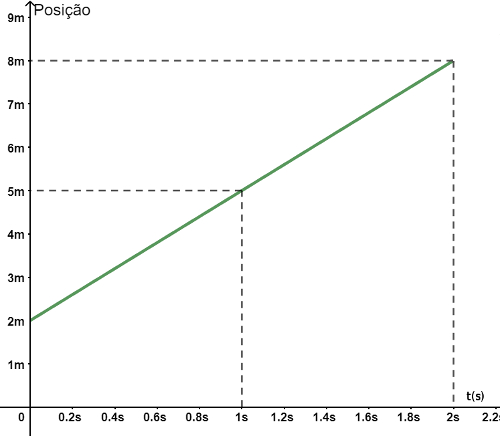
\includegraphics[width=0.3\textwidth]{grafico-de-posicao-movimento-uniforme-exercicio-1.jpg}
        \label{fig:ex_1}
    \end{figure}
    
    \begin{enumerate}
        \item 3 m/s
        \item 2 m/s
        \item 4 m/s
        \item 30 m/s
        \item 10 m/s
    \end{enumerate}
    
    \item Os dois primeiros colocados de uma prova de 100 m rasos de um campeonato de atletismo foram, respectivamente, os corredores A e B. O gráfico representa as velocidades escalares desses dois corredores em função do tempo, desde o instante da largada (t = 0) até os instantes em que eles cruzaram a linha de chegada.
    
    \begin{figure}[h]
        \centering
        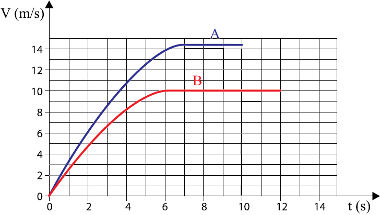
\includegraphics[width=0.5\textwidth]{grafico-corredores.jpg}
        \label{fig:ex_2}
    \end{figure}
    
    Analisando as informações do gráfico, é correto afirmar que, no instante em que o corredor A
cruzou a linha de chegada, faltava ainda, para o corredor B completar a prova, uma distância,
em metros, igual a:
    
    \begin{enumerate}
        \item 5
        \item 25
        \item 15
        \item 20
        \item 10
    \end{enumerate}
    
    \item Em uma prova de 100 m rasos, o desempenho típico de um corredor padrão é representado pelo gráfico a seguir:
    
    \begin{figure}[H]
        \centering
        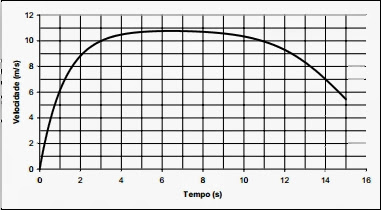
\includegraphics[width=0.5\textwidth]{BDQO.jpg}
        \label{fig:ex_3}
    \end{figure}
    Em que intervalo de tempo o corredor possui a aceleração máxima?
    
    \begin{enumerate}
        \item Entre 0 e 1s
        \item Entre 1 e 5s
        \item Entre 5 e 8s
        \item Entre 8 e 11s
        \item Entre 9 e 15s
    \end{enumerate}
    
    \item O famoso salto duplo twistcarpado de Daiane dos Santos foi analisado durante um dia de treinamento no Centro Olímpico em Curitiba, através de sensores e filmagens que permitiram reproduzir a trajetória do centro de gravidade de Daiane na direção vertical (em metros), assim como o tempo de duração do salto.
    
    \begin{figure}[H]
        \centering
        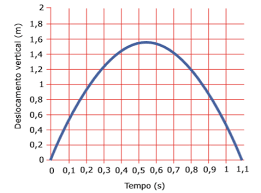
\includegraphics[width=0.5\textwidth]{download.png}
        \label{fig:ex_4}
    \end{figure}
    De acordo com o gráfico, determine:
    
    \begin{enumerate}
        \item A altura máxima atingida pelo centro de massa de Daiane;
        \item A velocidade média horizontal do salto, sabendo-se que a distância percorrida nessa direção é de 1,3m;
        \item A velocidade vertical de saída do solo. (\textit{Dica - use a Eq. de Torrcelli para resolver e caso necessário, adote g=10 m/s$^2$.})
    \end{enumerate}
    
    \item A posição de um automóvel em viagem entre duas cidades foi registrada em função do tempo. O gráfico a seguir resume as observações realizadas do início ao fim da viagem.
    
    \begin{figure}[H]
        \centering
        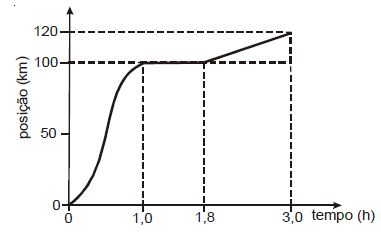
\includegraphics[width=0.5\textwidth]{unnamed.jpg}
        \label{fig:ex_6}
    \end{figure}
    
    \begin{enumerate}
        \item Indique durante quanto tempo o carro permaneceu parado.
        \item Calcule a velocidade escalar média do carro nessa viagem.
    \end{enumerate}
    
    \item O gráfico na figura descreve o movimento de um caminhão de coleta de lixo em uma rua reta e plana, durante 15s de trabalho.
    
    \begin{figure}[H]
        \centering
        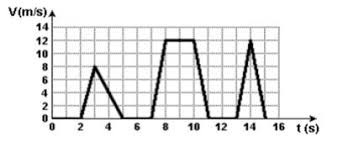
\includegraphics[width=0.5\textwidth]{ex_7.jpg}
        \label{fig:ex_7}
    \end{figure}
    
    \begin{enumerate}
        \item Calcule a distância total percorrida neste intervalo de tempo.
        \item Calcule a velocidade média do veículo.
    \end{enumerate}
    
    \item No instante t = 0 , o motorista de um carro que percorre uma estrada retilínea, com velocidade constante de 20 m/s, avista um obstáculo 100 m a sua frente.
    
    O motorista tem um tempo de reação t = 1 s, após o qual aciona os freios do veículo, parando junto ao obstáculo. Supondo-se que o automóvel tenha uma desaceleração constante, determine qual dos gráficos abaixo melhor representa a velocidade do automóvel desde o instante em que o motorista avista o obstáculo até o instante em que o automóvel pára.
    \begin{figure}[H]
        \centering
        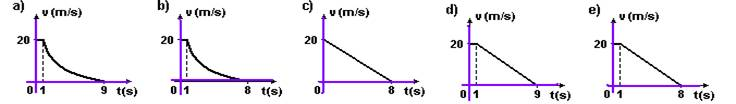
\includegraphics[width=\textwidth]{ex_8.jpg}
        \label{fig:ex_8}
    \end{figure}
    
    \item Considere os gráficos a seguir:
    \begin{enumerate}[I.]
            \item Espaço em função do tempo.
            \item Velocidade em função do tempo.
            \item Aceleração em função do tempo.
    \end{enumerate}
    
    \begin{figure}[H]
        \centering
        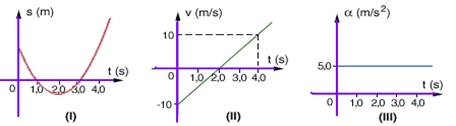
\includegraphics[width=0.7\textwidth]{i_a7a9ebcce6cda076_html_4c31708 (1).jpg}
        \label{fig:ex_9}
    \end{figure}
    A respeito desses gráficos é correto afirmar que:
    
    \begin{enumerate}
        \item Somente I e II podem representar o mesmo movimento. 
        \item Somente I e III podem representar o mesmo movimento.
        \item Somente II e III podem representar o mesmo movimento.
        \item Os três gráficos podem representar o mesmo movimento.
        \item Cada gráfico representa um movimento distinto.
    \end{enumerate}
    
    \item  Ao abrir uma garrafa de refrigerante com gás, muitas bolhas de gás carbônico ali formadas sobem desde o fundo da garrafa com um movimento acelerado. Supondo-se que as bolhas têm o mesmo tamanho e a mesma quantidade de gás durante toda subida e desprezando-se quaisquer perdas de energia por resistência ao movimento. Dos gráficos a seguir aqueles que representam, respectivamente, a posição e a velocidade das bolhas são:
    
    \begin{figure}[H]
        \centering
        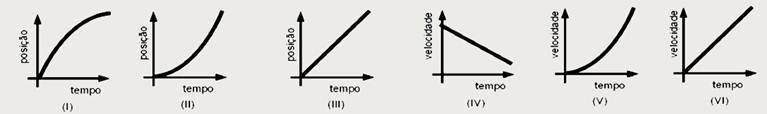
\includegraphics[width=0.9\textwidth]{last.jpg}
        \label{fig:ex_9}
    \end{figure}
    
    \begin{enumerate}
        \item I e IV
        \item I e VI
        \item II e V
        \item II e VI
        \item III e V
    \end{enumerate}
\end{enumerate}
\newpage
\section{GABARITO}

\begin{enumerate}
    \item (a)
    \item (d) - aqui o que tem que se feito é calcular a área debaixo do gráfico B a partir do tempo que o A termina - 10s. Como ele está a uma velocidade de 10 m/s e demora mais 2s do que o A para terminar, então ele faltava: $\Delta S = v*\Delta t = 10 * 2 = 20m $.
    
    \item (a) - lembrar que aceleração é a variação de velocidade, seja aumentar ou diminuir. A velocidade cresce/decresce o máximo entre 0 e 1s.
    
    \item
    \begin{enumerate}
        \item A altura máxima, pelo gráfico é de, aproximadamente, 1,55 m.
        \item Como pelo gráfico, ela demorou 1,1 segundo para fazer o pulo e a distância percorrida horizontalmente é de 1,3m: 
        \begin{equation}
            v = \frac{\Delta S}{\Delta t} = \frac{1,3}{1,1} \approx 1,2 m/s
        \end{equation}
        
        \item Usando a Equação de Torricelli para quando ela sai do chão e chega no ápice do salto (ou seja, v=0) e lembrando que ela saltou para cima, então temos a aceleração da gravidade atuando, temos que:
        \begin{equation}
            \begin{split}
                v^2 = v_0^2 + 2a\Delta S\\
                0 = v_0^2 + 2*(-10)*1,55 \quad \text{\Delta S = 1,55 porque é a altura máxima, pelo gráfico, e é o ápice do salto} \\
                v0_^2 = 31 \implies v_0 \approx 5,6 m/s
            \end{split}
        \end{equation}
    \end{enumerate}
    
    \item
    \begin{enumerate}
        \item Ele ficou parado entre 1,0 a 1,8 s, logo ele ficou parado por 0,8s.
        \item A velocidade média é dada por:
        \begin{equation}
            \begin{split}
                v = \frac{\Delta S}{\Delta t} \\
                v = \frac{120}{3} = 40 \frac{km}{h}
            \end{split}
        \end{equation}
    \end{enumerate}
    
    \item \begin{enumerate}
        \item A distância total percorrida é a soma das 3 áreas debaixo do gráfico.
        
        \begin{equation}
            \Delta S_{total} = \Delta S_1 + \Delta S_2 + \Delta S_3
        \end{equation}
        
        em que $\Delta S_1$ é a área do triângulo entre 2 e 5s, $\Delta S_2$ é a área do trapézio e $\Delta S_3$ é a área do outro triângulo. Calculando as áreas dessas figuras, temos que:
        
        \begin{equation}
            \Delta S_{total} = 12 + 36 + 12 = 60 m
        \end{equation}
        
        \item A velocidade média do veículo é dada por:
        
        \begin{equation}
            \begin{split}
                v = \frac{\Delta S_{total}}{\Delta t} \\
                v = \frac{60}{15} = 4 m/s
            \end{split}
        \end{equation}
    \end{enumerate}
    
    \item (d)
    
    \item (d)
    
    \item (d)
\end{enumerate}
\end{document}
